\documentclass[a4paper, 10pt, final, garamond]{book}
\usepackage{cours-preambule}

\titleformat{\item}{}{\arabic{item})}{.5em}{}{}
\titleformat{\subitem}{}{\arabic{item}) \alph{subitem} --}{.5em}
{}{}

\makeatletter
\renewcommand{\@chapapp}{Devoir surveill\'e -- num\'ero}
\makeatother

\begin{document}
\setcounter{chapter}{3}

\chapter{Commentaires sur le DM n\degree4}

\begin{NCprop}[width=\linewidth]{\centering\bfseries\ Rappel des malus}
    Chacune des lettres suivantes sur vos copies sont des malus de \num{1}
    point.\smallbreak
    \begin{minipage}{0.50\linewidth}
        \begin{itemize}
            \item A~: application numérique mal faite~;
            \item V~: confusion ou oubli de vecteurs~;
            \item P~: prénom sur copies manquant~;
            \item N~: numéro copie manquant~;
        \end{itemize}
    \end{minipage}
    \begin{minipage}{0.50\linewidth}
        \begin{itemize}
            \item U~: unité manquante ou mauvaise~;
            \item H~: homogénéité non respectée~;
            \item $\f$~: loi physique fondamentale brisée.
        \end{itemize}
    \end{minipage}
\end{NCprop}

\begin{enumerate}
    \item RAS.
    \item Points pour $\Ec_c = \frac{1}{2}mv_m{}^2$ et $\Ec_c =
        \frac{1}{2}Mv_M{}^2$.
    \item \textbf{À partir des relations entre force et énergie~!!}
    \item 
        \[\Huge \dv{\Ec_p}{\boxed{\tt}}\]
    \item RAS
    \item «~C'est évident~» n'est pas une réponse…
    \item Attention à vos développements de \textsc{Taylor}. C'est pas parce
        qu'on fait de la physique qu'on peut passer outre toute la rigueur des
        mathématiques. Notamment, si vous utilisez «~=~», il faut le $o(\tt^2)$.
        Si vous utilisez $\sim$, non. S'il est écrit «~en fonction de $M_0$ etc,
        la réponse ne peut pas contenir $\tt_{\eq,1}$~! Attention à l'énoncé.
    \item Calculer $\Ec_m$ avant de dériver. $\tp$ non toujours nul, donc on
        peut simplifier.
    \item RAS. Il faut savoir résoudre.
    \item À revoir pour la plupart. Questions «~faciles~» (comprendre «~pas
        calculatoires~»), mais plein de points.
    \item Il n'est pas choquant d'avoir une énergie mécanique nulle~!
    \item Attention à la terminologie aussi.
\end{enumerate}

\begin{center}
    \bfseries\Large
    Bonus
\end{center}

Vous savez comment on trouve que des valeurs ont été truquées~? On vérifie leur
distribution théorique. Vous savez ce qu'est la distribution théorique de notes
à des élèves~? Comme toute grandeur à grand échantillon, une gaussienne.
Regardez la distribution de notes suivantes~: est-ce une gaussienne~?

\begin{center}
    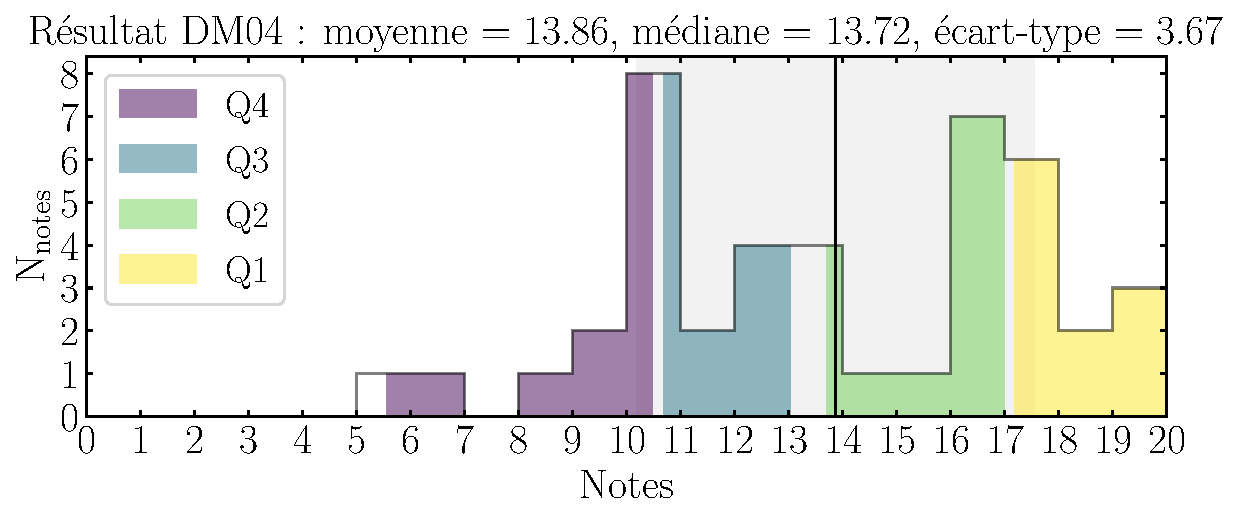
\includegraphics[width=.8\linewidth]{res_DM04.pdf}
\end{center}

Donc clairement la formule des DMs va bientôt changer~: il y a beaucoup trop de
scribes et pas assez de scientifiques dans cette classe.

\end{document}
